
\begin{defn}
Se llama \emph{ funci\'on polinomial} o  \emph{ polinomio} con coeficientes $a_0, a_1, ..., a_n\in \R$ a la funci\'on $p:\R \longrightarrow \R$ que a cada $x\in \R$ le asigna el valor:
\[
p(x)=\sum_{i=0}^n a_ix^i=a_0+a_1x+a_2x^2+\cdots +a_nx^n.
\]
Esta expresión es la forma canónica de un polinomio.
\begin{itemize}
\item El \emph{grado de un polinomio}, que dentamos $gr(p)$, es el mayor valor $n$ tal que $a_n\ne 0$, en tal caso, $a_n$ es llamado \emph{coeficiente principal}. Si el coeficiente principal es igual a 1, entonces el polinomio se dice \emph{m\'onico}.
\item El polinomio constante igual a 0 se llama  polinomio nulo, se denota $\theta(x)$ y se conviene que no tiene grado.
\item El coeficiente $a_0$ se denomina \emph{t\'ermino libre,  independiente} o coeficiente de posición.
\item Se denota por $\mathcal{P} ( \R)$ al conjunto de todos los polinomios con coeficientes en $\R$.
%Por ejemplo, $ \mathcal{P} (\Q), \mathcal{P}(\R)$ \'o $\mathcal{P}(\C)$.
\end{itemize}
\end{defn}

Las funciones potncia son casos particulares de polinimios, se distinguen en que tienen un solo término.
Ejemplos de polinomios son:

\begin{itemize}
\item Polinomio constante: $p(x)=-0.3$.
\item Recta: $p(x)= 2x-4$.
\item Parábola: $p(x)= 3x^2-4x+1$.
\item Polinomio de grado superior a 2: $p(x)= -x^5+2x^2-x$.
\end{itemize}

En general cualquier función que se exprese solo con suma, resta y multiplicación de constantes por potencias de $x$ es un polinomio, por ejemplo:

$$p(x)=x(x^2+3)-(2x-5)(0.5+2x)$$
 es un polinomio, pero no está en su forma canónica. Para poder conocer el grado y coeficientes del polinomio debemos primero llevarlo a su forma canónica.
 
 \begin{eqnarray*}
 p(x)&=&x(x^2+3)-(2x-5)(0.5+2x)\\
 &=&x^3+3x-x+2.5-4x^2+10x\\
 &=&x^3-4x^2+12x+2.5
 \end{eqnarray*}
 
 Recién entonces podemos ver que es de grado 3, su coeficiente principal es 1 y su término libre es 2,5.
 La igualdad de polinomios se puede evidenciar solo en la forma canónica.
 


\bigskip

\begin{defn}
Decimos que dos polinomios 
$$p(x)=\sum_{i=0}^n a_ix^i,\qquad q(x)=\sum_{i=0}^n b_ix^i, $$
son iguales si 
$$ gr(p)=gr(q) \wedge \forall i\in\{1,\dots,gr(p)\},\ a_i=b_i.$$
\end{defn}

Cuando estudiamos las parábolas, fue importante identificar sus raíces, esto es, los valores de $x$ en los cuales la función toma el valor 0, o en otras palabras, los puntos donde la función intersecta al Eje X.
Este problema tendrá relevancia en los polinomios en general, aunque será mucho más difícil resolverlo cuando el grado es mayor o igual a 3.

\medskip

\begin{defn}
Sean  $p \in \mathcal{P}(\R)$ y $c\in \R$, se dice que   $c$ es  una {  {\bf ra{\'\i}z o cero}}  de  $p$ si $p(c)=0$. Es decir, si:
$$p(c)=\sum_{i=0}^n a_ic^i=a_0+a_1c+a_2c^2+\cdots +a_nc^n=0.$$
\end{defn}

El valor $x=c$ corresponde a la intersecci\'on de la gr\'afica de $p$ con el eje $X$.


\section{Operaciones}

En el conjunto de los polinomios, consideramos las dos operaciones clásicas de suma y multiplicación de funciones. 
Dada la forma simple de los polinomios, podemos describir estas funciones de manera simplificada, y determinar algunas de sus propiedades.

\subsection{Suma}

Se considera la operación de suma de funciones, lo cual en el caso de los polinomios se traduce en que sus respectivos coeficientes se suman uno a uno.

\medskip

\begin{defn}
 Si tenemos dos polinomios $p(x)=\sum_{i=0}^n a_ix^i$, $q(x)=\sum_{i=0}^m b_ix^i $, donde, sin pérdida de generalidad, y gracias a la conmutatividad de la suma en $\R$, podemos asumir que $n\ge m$.

$$p(x)+q(x)=\sum_{i=0}^{m} (a_i+b_i)x^i+\sum_{i=m+1}^n a_ix^i. $$
\end{defn}

Así vemos que $gr(p+q)\le\max\{gr(p)+gr(q)\}$, o simplemente $gr(p)$ cuando $q=\theta$.
Cuando los dos polinomios tiene el mismo grado la desigualdad podría ser estricta si es que se cancelan los coeficientes principales, por ejemplo $(3x^3-2x^2+x-4)+(-3x^3+2x^2+5x+2)=6x-2$ y su grado es 1 en lugar de 3.

La suma hereda la conmutatividad y asociatividad de la suma en $\R$, así mismo, el polinomio nulo, $\theta$ es neutro para la suma ya que:

$\forall x\in\R,\ p(x)+\theta(x)=p(x)+0=p(x).$

También tenemos que el opuesto aditivo de un polinomio, se obtiene simplemente tomando el opuesto aditivo de cada uno de sus coeficientes, o dicho de otra manera, ponderando el polinomio completo por $-1$.

\subsection{Multiplicación}
De igual manera, se considera la multiplicación de funciones, la cual da lugar a una fórmula algo más complicada.

\medskip

\begin{defn}
 Si $p(x)=\sum_{i=0}^n a_ix^i,\qquad q(x)=\sum_{i=0}^m b_ix^i $, donde $n\ge m$, entonces:
$$p(x)\cdot q(x)=\sum_{k=0}^{m} \left(\sum_{i=0}^ka_{k-i}b_{i}\right)x^k
+\sum_{k=m+1}^{n} \left(\sum_{i=0}^ma_ib_{k-i}\right)x^k
+\sum_{k=n+1}^{n+m} \left(\sum_{i=k-n}^ma_ib_{k-i}\right)x^k. $$
\end{defn}

De esta definición se concluye que $gr(pq)=gr(p)+gr(q)$, y si $p=\theta$ o $q=\theta$, entonces $pq=\theta$.

Observamos que la multiplicación de polinomios también hereda la conmutatividad y asociatividad de la multiplicación en $\R$.
El neutro multiplicativo es el polinomio constante igual a 1, es decir, el polinomio de grado 0 que vale 1 en todas partes.

En general NO existe inverso multiplicativo, ya que la función $\frac{1}{p}$ solo es un polinomio, cuando $p$ es de grado 0.

Justmente la fórmula $gr(pq)=gr(p)+gr(q)$ nos dice que si hubiera un polinomio $q$ tal que $pq=1$, entonces se tendría que tener $gr(q)=-gr(p)$, pero el grado es siempre un entero no negativo, por lo tanto, solo los polinomios de grado 0, los polinomios constantes, tiene inverso multiplicativo.

De manera análoga, podemos ver que la multiplicación de polinomios hereda otra importante propiedad de la multiplicaición en un cuerpo:

$$p\cdot q=\theta \Longrightarrow (p=\theta \vee q=\theta)$$

Para ver esto suponemos que $p$ y $q$ son no nulos, entonces tiene grado mayor o igual a 0, por lo tanto, $gr(pq)=gr(p)+gr(q)\ge 0$, así $pq$ no puede ser nulo.

Finalmente, la multiplicación de polinomios hereda la distributividad con respecto a la suma de polinomios de la distributividad en $\R$. 
Así, podemos resumir las propiedades de las operaciones de suma y multiplicación en el siguiente cuadro.

\begin{center}
\begin{tabular}{| l p{7.5cm} | l p{5.5cm} |}
\hline
S1).&$(p+q)+r=p+(q+r).$ & S2).& $p+q=q+p.$    \\
\hline
 S3). & El polinomio nulo es tal que $p+\theta=p$& S4).& $\exists  -p\in  \R[x]:p+(-p)=\theta $\\
\hline
M1).& $(p\cdot q)\cdot r=p\cdot(q\cdot r)$&M2).& $p\cdot q =q \cdot p$\\
\hline
M3). &El polinomio $1$ es tal que $p\cdot 1=p$ &N). & $p\cdot q=\theta \Longrightarrow p=\theta$ o $q=\theta$\\
\hline
D).& $p\cdot (q+r)=p\cdot q+p
\cdot r$ &{}&{}\\
\hline
\end{tabular}
\end{center}

Estas propiedades corresponden a una estructura de \emph{Anillo conmutativo con unidad y sin divisores de cero}, propiedad que comparte  con el conjunto de los n\'umeros enteros. 
En el siguiente capítulo veremos que tiene muchas más cosas en común.

\section{División Euclidiana}

El siguiente teorema define la llamada división {\bf Euclidiana}, en la cual se busca un polinomio cuociente, y se especifica la parte restante que no se pudo dividir.

\medskip

\begin{thm}
Si $p, d \in \mathcal{P}(\R)$ son dos polinomios tales que $gr(p)\ge gr(d)$  y $d\ne \theta$, entonces existen  \'unicos polinomios $q, r \in \mathcal{P}(\R)$, llamados  respectivamente {\bf cuociente y resto},  tales que:
$$p=q  d +r,\quad \hbox{ y}  \quad (r=\theta \quad  \hbox{ o }  \quad  gr(r) <gr(d)).$$
\end {thm}

Notamos que el resto $r$ está definido tal que su grado sea estrictamente inferior al grado de $d$, o bien que sea el polinomio nulo.

Del  teorema se tiene que 
$$\frac{p}{d}=q+\frac{ r}{d}.$$

Donde la propiedad que destacamos nos dice que $\frac{r}{d}$ es una función que tiende a 0 cuando $|x|$ crece, e decir que tiende asintóticamente a 0.

Esta escritura permite visualizar mejor la función racional $\frac{p}{d}$.

\medskip

\begin{ejemplo}
Por ejemplo, el cuociente y resto de dividir $p(x)=6x-x^2+4x^3+5x^4$ por $d(x)=x^2+1$ lo podemos calcular por el siguiente procedimiento.

    \[
    \begin{array}{rrrrrlll}
        &5x^4 & + 4x^3 &- x^2 &+ 6\,x&+0:& (x^2 + 1)= & 5x^2 + 4x - 6\\
        -&(5x^4 &&+ 5x^2)&&&&\\
        \cline{1-4}
        &&4x^3&+6x^2&+6\,x&&&\\
        &-&(4x^3&&+4x)&&&\\
        \cline{2-5}
        &&&-6x^2&+2x&&&\\
        &&-&(-6x^2 &&-6)&&\\
        \cline{3-6}
        &&&&2x&+6&&
    \end{array} 
    \]

Así,  $q(x)=5x^2+4x-6$ y $ r(x)=2x+6$.


Esto significa que
$$\frac{6x-x^2+4x^3+5x^4}{x^2+1}=5x^2+4x-6+\frac{2x+6}{x^2+1},$$
de donde podemos visualizar su gráfico (en azul) como una suma de una parábola (en verde) más una función racional que se hace despreciable en los extremos\footnote{Dibujo hecho mediante el software gratuito Geogebra.}.

\begin{center} 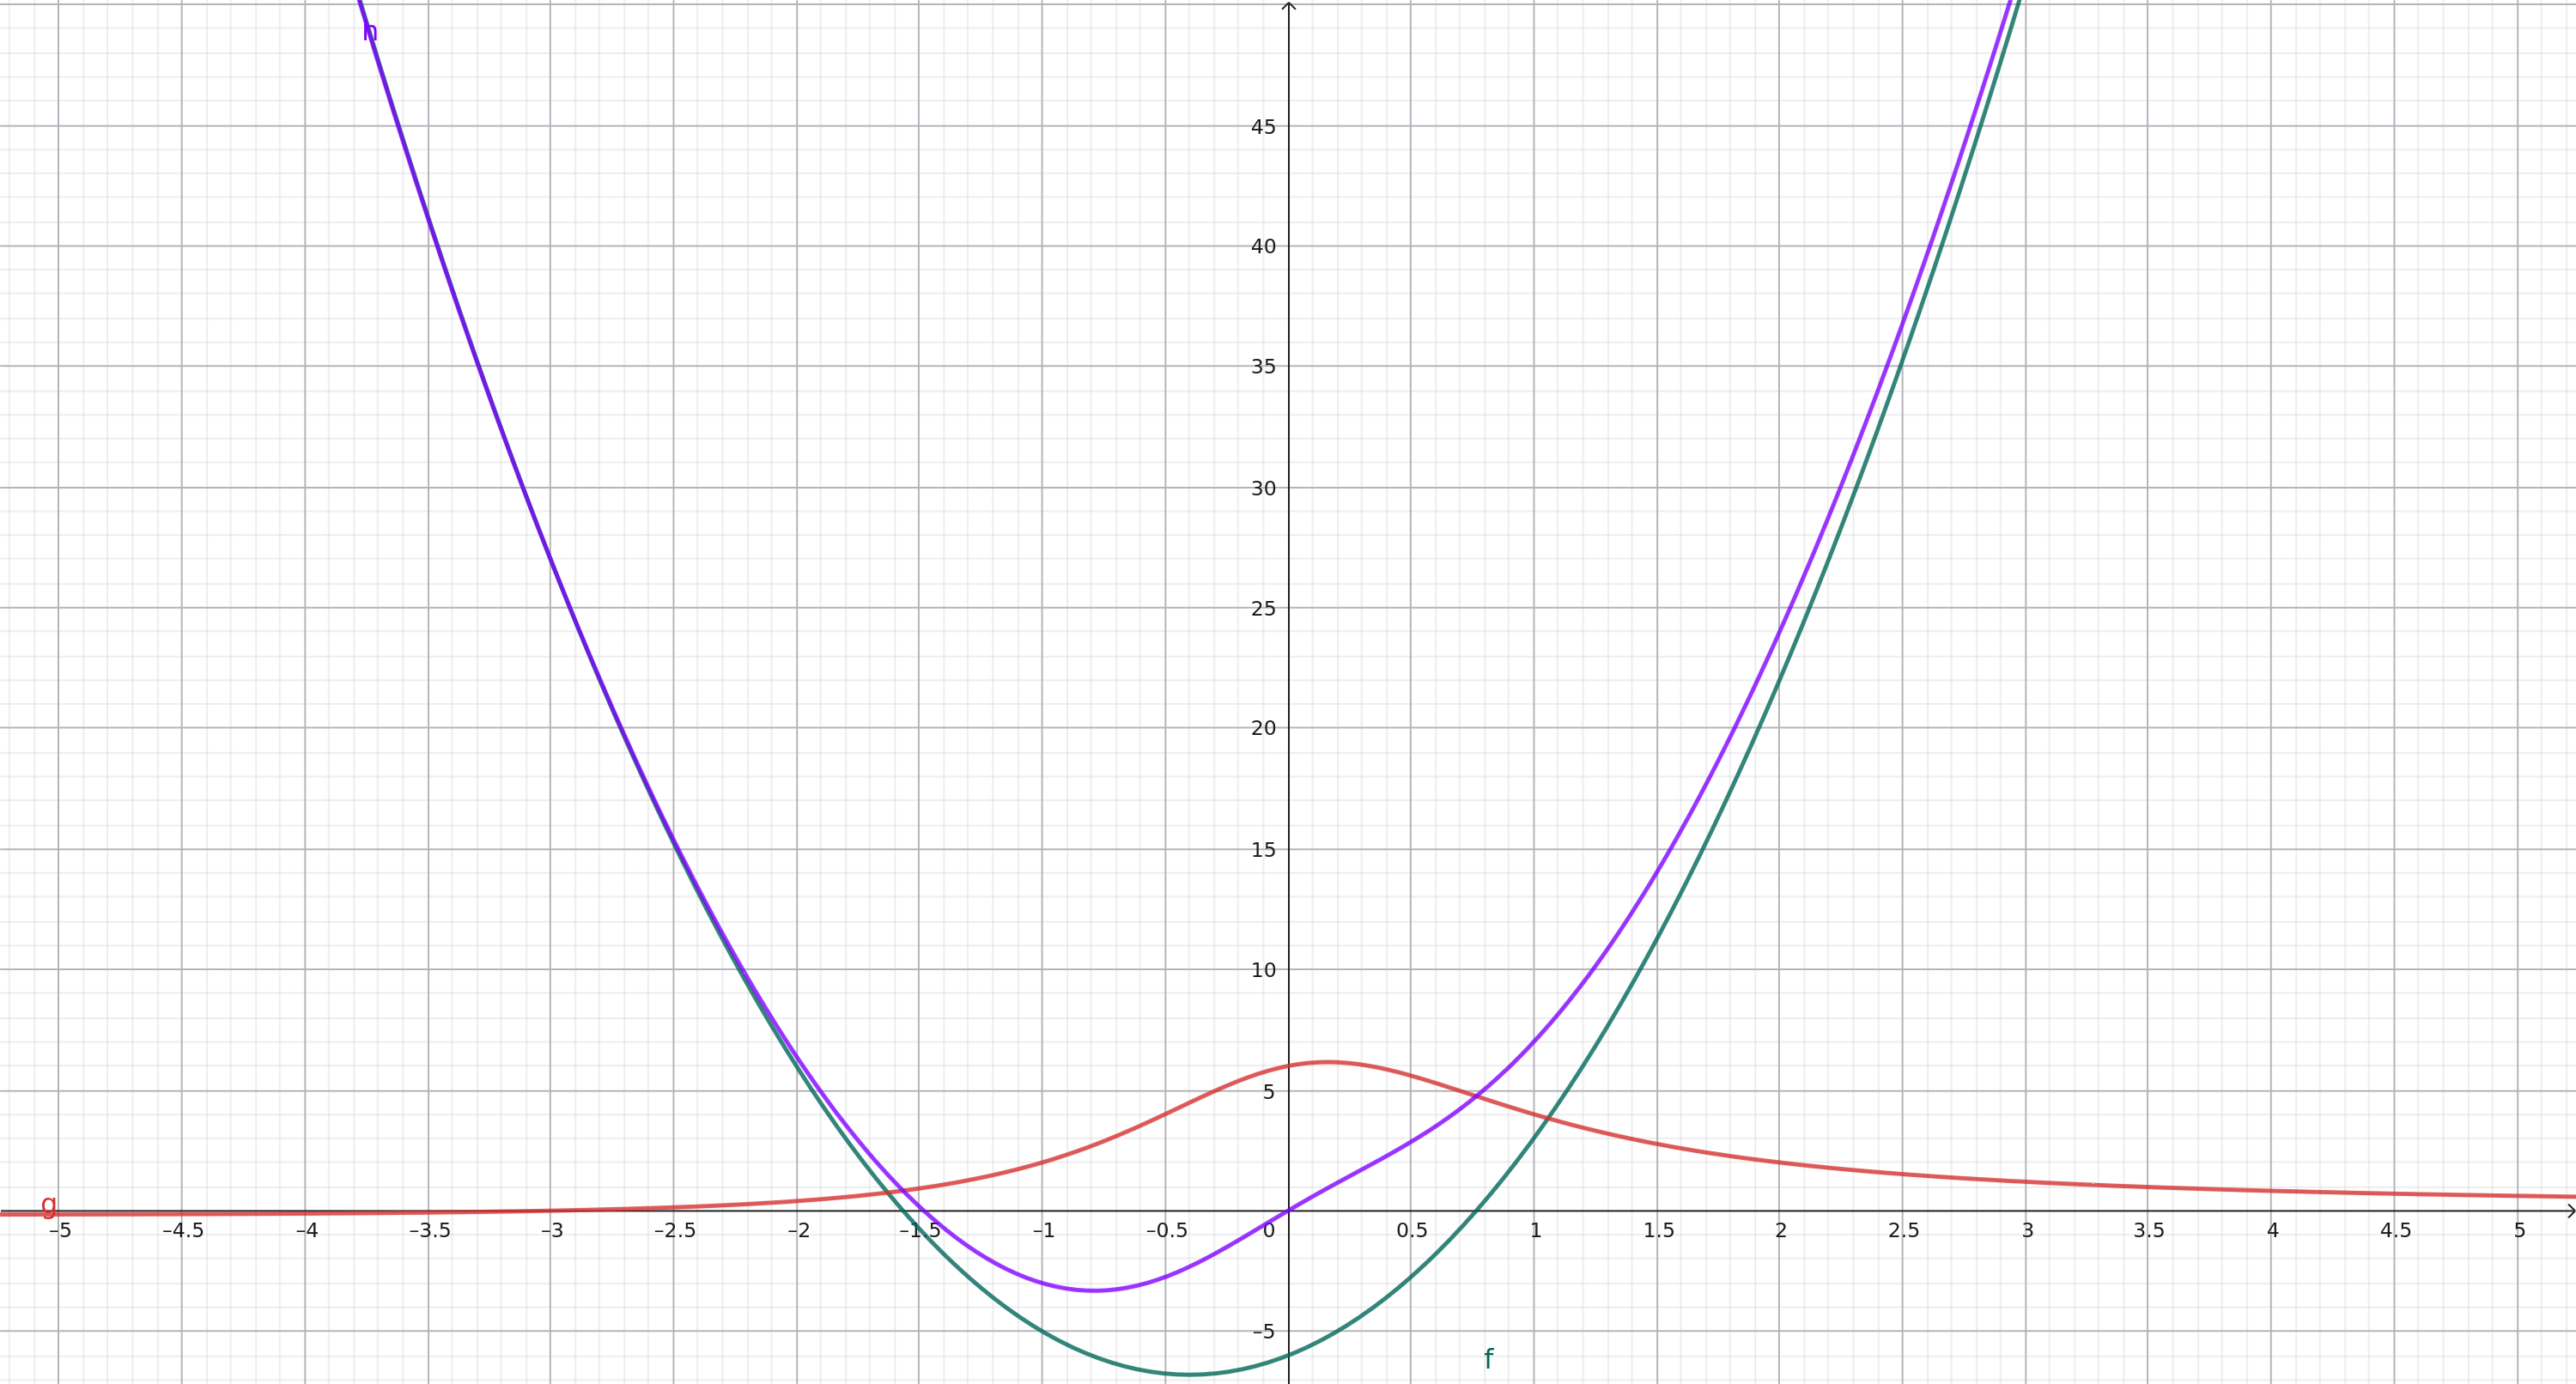
\includegraphics[height=6cm]{racional.png}
\end{center}
\end{ejemplo}

\section{Descomposición en factores irreducibles}

En esta sección desarrollamos más la analogía entre el conjunto de los números enteros y el de los polinomios.

\subsection{Divisibilidad}

\begin{defn}
Si $r=\theta$, entonces decimos que {\bf $q$ divide a $p$} y que {\bf $p$ es divisible por $d$}.
En otras palabras, decimos que $d$ divide a $p$ si existe un polinomio $q$ tal que 
$$p=rd.$$
\end{defn}

Esta noción de divisibilidad es análoga a la divisibilidad de números enteros, y nos conduce a una noción análoga a la de primalidad.

\subsection{Irreducibilidad}

\begin{defn}
Un polinomio $p$ de grado mayor o igual a 1 se dice  {\bf reducible} en $\mathcal{P}(\R)$ si existen dos polinomios $q, s\in \mathcal{P}(\R)$, con $gr(q)\ge 1$ y $ gr(s)\ge 1$, tales  que $p=q s$.

En caso contrario se dice que $p$ es {  {\bf irreducible o primo}} en $\mathcal{P}(\R)$.
\end{defn}


Notamos la importancia de pedir que los grados de $q$ y $s$ sean mayores o iguales a 1, ya que si $q$ o $s$ tuvieran grado 0, serían polinomios constantes, y todos los polinomios se pueden siempre escribir como multiplicación de un polinomio constante por otro polinomio, por ejemplo:

$$ x^2+2=\frac{1}{5}\cdot (5x^2+10),$$

Así, si $p$ es reducible, entonces $gr(p)=gr(q)+gr(s)\ge 2$, todos los polinomios reducibles tienen grado mayor o a igual a 2.

\medskip

\begin{rem}
 Los polinomios de grado 1, $p(x)=a_0+a_1x$,  son todos irreducibles.
\end{rem}

\subsection{Teorema de descomposición prima}

\begin{thm}[{Teorema de descomposición prima.}]
Todo polinomio  $\displaystyle p(x) \in \mathcal{P}(\R)$ admite una única descomposici\'on como producto de polinomios irreducibles mónicos, es decir, existen únicos $p_1, p_2,...,p_m\,\in\R$ mónicos irreducibles y $C\in \R$ tales que:
\[
p(x)=Cp_1(x)p_2(x)\cdots p_m(x);
\]
\end{thm}

Al igual que el teorema análogo que se tiene en los números naturales, este teorema es extremadamente útil, y de él se desprenden varias consecuencias.
Para comenzar, observamos que los divisores de un polinomio, son todos parte de su descomposición única en polinomios irreducibles.

\subsection{Teorema del Factor}

La principal consecuencia de esto tiene relación con las raíces de $p$. Tenemos que $p(x)$ será igual a 0, si y solo sí existe $i\in\{1,\dots,m\}$ tal que $p_i(x)=0$, en otras palabras, $x$ es raíz de $p$ si y solo si $x$ es raíz de alguno de los factores de $p$.
Esto da lugar a los siguientes corolarios.

\medskip

\begin{cor}
Si $p$ es irreducible en $\mathcal{P}(\R)$, entonces  no tiene raíces reales o bien es de grado 1 y tiene una sola.
\end{cor}

De lo anterior deducimos que todas las raíces de un polinomio son raíces de alguno de sus factores irreducibles de grado 1, de donde se obtiene el siguiente teorema.

\medskip

\begin{thm}[Teorema del Factor]
Un polinomio $p$ tiene a $c$ como raíz si y solo si el polinomio $d(x)=x-c$ es factor de $p$.
\end{thm}

En otras palabras:
\begin{eqnarray*}
p(c)=0 &\Longleftrightarrow& \exists\, q\in  \mathcal{P}(\R),\ \forall x\in \R,\  p(x)=q(x)(x-c).\\
&\Longleftrightarrow&d(x)=x-c\textrm{ divide a } p
\end{eqnarray*}

Si analizamos el grado de $p$ y usamos el teorema de descomposición única, obtenemos lo siguiente:

$$ gr(p)=\sum_{i=1}^m gr(p_i).$$

Dado que cada raíz está asociada a al menos un factor de grado 1, obtenemos el siguiente corolario.

\medskip

\begin{cor}
Un polinomio $p$ tiene a lo m\'as $gr(p)$ ra{\'\i}ces distintas.
\end{cor}

El cual, a su vez, nos lleva al siguiente corolario.

\medskip

\begin{cor}
Si dos polinomios $p$ y $q$, de grado $n$, coinciden en $n+1$ puntos distintos, entonces son iguales: $p=q$. 
\end{cor}



\subsection{Multiplicidad de una raíz}

Ahora bien, el factor $d(x)=x-c$ puede figurar en la descomposición única de $p$ con un exponente mayor a 1.
Sea $k\in \N$ el mayor natural tal que $(x-c)^k$ divide a $p$.
Es decir, tomemos $q \in \mathcal{P}(\R)$ no divisible por $(x-c)$ tal que 

\vspace{-.3cm}

$$\forall x\in \R, \quad p(x)=q(x)(x-c)^k.$$

\vspace{-.1cm}

En tal caso decimos que \emph{$c$ es una ra\'iz de multiplicidad $k$.}
Si $k=1$ se dice que $c$ es una {\bf ra\'iz} simple.

\medskip

\begin{rem}
La suma de las multiplicidades de todas las ra\'ices de $p$ es menor o igual que $gr(p)$.
\end{rem}


\section{Teorema del resto}

La división Euclidiana es particularmente interesante cuando dividimos por un polinomio de grado 1, ya que en ese caso, el resto, al tener grado 0 no ser nulo, es una constante. 
El siguiente teorema expresa esto detallando la constante en cuestión.

\medskip

\begin{thm}
El resto de dividir  $p \in \mathcal{P}(\R)$ por  $(x-c)$ es $p(c)$.
\end{thm}

La demostración es interesante, si $q$, $r$ son el cuociente y el resto de dividir $p$ por $x-c$, respectivamente, entonces, por lo dicho antes, $r(x)=a$, con $a$ una constante en $\R$.
Así:
$$ p(x)=q(x)(x-c)+a,$$
y
$$ p(c)=q(c)(c-c)+a=0+a=a.$$
Es decir, la constante $a$ es igual al valor de $p$ en $c$.

Si $c$ es una raíz de $p$, entonces $a=0$, y $(x-c)$ divide a $p$ (como ya habíamos discutido).

Si $c$ no es raíz de $p$, el teorema de todas formas nos sirve para conocer el valor de $p$ en $c$, evaluar el polinomio $p$ en $x=c$, y resulta que hacer la división Euclidiana de $p$ en $(x-c)$ puede ser una forma computacionalmente eficiente de evaluar $p$ en $c$, conocida como Método de Ruffini o división sintética.

\section{Localización de raíces en $\R$}

El siguiente teorema no se puede demostrar con las herramientas que hemos visto en este curso, pero es de gran utilidad, pues nos acota el espacio donde buscar las raíces de $p$.
En general estas raíces las buscaremos mediante métodos computacionales iterativos que solo podrán darnos un valor aproximado de la raíz, y para ello es muy importante saber de antemano en qué intervalo debemos buscar las raíces, este teorema nos da justamente eso.

\begin{thm}
Si $c\in \R$ es ra{\'\i}z de $\displaystyle p(x)=\sum_{i=0}^n a_ix^i$, con $a_0,\dots,a_n\in\R$, entonces:
$$\frac{|a_0|}{\alpha+|a_0|}\le |c|\le \frac{\beta+|a_n|}{|a_n|},$$
donde:
$\alpha=$m\'ax$\{|a_n|,...,|a_1|\}$ y $\beta=$m\'ax$\{|a_{n-1}|,...,|a_0|\}$.
\end{thm}

\medskip

\begin{ejemplo}
Si aplicamos este teorema al polinomio $p(x)=x^3-3x^2-x+3$, vemos que $\alpha=1$, $\beta=3$, $a_0=3$, $n=3$ y $a_n=1$, por lo tanto  $\frac{1}{2} \le |c| \le 4$; todas las raíces de $p$ se encuentran en $[-4,-\frac{1}{2}]\cup[\frac{1}{2},4]$.
\end{ejemplo}



\section{Raíces complejas de un polinomio a coeficientes reales}

Aunque $p$ tenga coeficientes reales, podemos aplicarlo a valores complejos, es decir, verlo como una función $p:\C\rightarrow \C$.
Allí también nos va a interesar qué valores complejos hacen que $p$ se anule, es decir, nos van a interesar sus \emph{raíces complejas.}

\medskip

\begin{thm}
Sea  $p \in \mathcal{P}(\R)$,  y $z=a+bi\in \C$ (con $a,b\in\R$ y $b\not = 0$). Si $p(z)=0$, entonces $p(\overline{z})=0$ y existe $q\in  \mathcal{P}(\R)$  tal que 
$$\forall\,x\in\R,\ p(x)=q(x)[(x-a)^2+b^2].$$
\end{thm}

En efecto, si $p(x)=\sum_{i=0}^n a_ix^i$, con $a_0,\dots,a_n\in\R$, entonces, como $p(z)=0$:

\begin{eqnarray*}
0&=&\overline{0}\\
&=&\overline{p(z)}\\
&=&\overline{\sum_{i=0}^n a_iz^i}\\
&=&\sum_{i=0}^n \overline{a_iz^i}\\
&=&\sum_{i=0}^n a_i\overline{z^i}\\
&=&\sum_{i=0}^n a_i\overline{z}^i\\
&=&p(\overline{z}).
\end{eqnarray*}

Entonces $x-z$ y $x-\overline{z}$ serían factores de $p$, con lo cual $(x-z)(x-\overline{z})$ es factor de $p$, pero
\begin{eqnarray*}
(x-z)(x-\overline{z})&=&(x-a-bi)(x-a+bi)\\
&=&((x-a)-bi)((x-a)+bi)\\
&=&(x-a)^2-(bi)^2\\
&=&(x-a)^2+b^2.
\end{eqnarray*}
De donde se concluye el teorema.

Dado que $(x-a)^2+b^2$ tiene dos raíces en $\C$, no puede tener raíces en $\R$, es un polinomio irreducible en $\R$.
Podemos desarrollarlo un poco más.

$$(x-a)^2+b^2=x^2-2ax+ (a^2+b^2)$$


\begin{rem}
Si $z=a+bi$ es una ra{\'\i}z compleja de $p$ de multiplicidad $k$, entonces $\overline{z}$ tambi\'en lo es, con la misma multiplicidad y el polinomio $[(x-a)^2+b^2]^k$ es un factor de $p$ de grado $2k$.
\end{rem}


\subsection{Teorema fundamental del álgebra}

El siguiente es el teorema más importante del capítulo. Su demostración requiere herramientas de cálculo complejo, y por lo tanto no podemos desarrollarla en este apunte.
Este teorema se refiere a polinomios cuyo coeficientes pueden ser reales o complejos.
Habíamos visto que en $\R$ existen polinomio que no tiene ninguna raíz real, por ejemplo $x^2 +1$.
Esto no ocurren en $\C$, todos los polinomios a coeficientes en $\C$ tienen al menos una raíz en $\C$.
Todas las ecuaciones polinomiales a coeficientes en $\C$ tienen soluciones en $\C$.

\medskip

\begin{thm}
Todo polinomio $p\in\mathcal{P}(\C)$ tiene al menos una raíz en $\C$.
\end{thm}

La principal consecuencia de esto es que en $\C$ los únicos polinomios irreducibles son los polinomios de grado 1.

Como $\R\subseteq \C$, podemos aplicar el teorema también a los polinomios a coeficientes en $\R$.


\medskip

\begin{thm}
Todo polinomio $p\in\mathcal{P}(\R)$ tiene al menos una raíz en $\C$.
\end{thm}

Del análisis anterior, sabemos que cada raíz compleja de $p\in\mathcal{P}(\R)$ arroja un factor de grado par de $p$, con lo cual, si  $p$ tiene grado impar, ha de tener al menos un factor $q$ de grado impar.

El teorema fundamental del álgebra nos dice que $q$ también tiene al menos una raíz, tal raíz es también raíz de $p$, y como ya hemos considerado todas las raíces complejas de $p$, concluimos que las raíces de $q$ han de ser toda reales, y al ser $q$ de grado impar, tiene grado mayor o igual a 1, con lo cual, tiene al menos una raíz.
Que es justo lo que afirma el siguiente corolario.

\medskip

\begin{cor}
 Si $p\in  \mathcal{P}(\R)$ tiene grado impar, entonces $p$ tiene al menos una ra{\'\i}z.
\end{cor}

\medskip

\begin{ejemplo}
Podemos descomponer $p(x)=x^6-1$ en factores irreducibles.
\[
\begin{array}{rl}
p(x)&=x^6-1\\
	&=(x^3-1)(x^3+1)\\
	&=(x-1)(x^2+x+1)(x+1)(x^2-x+1).
\end{array}
\]
Como $x^2+x+1$ y $x^2-x+1$ tienen ra\'ices complejas, concluimos que la descomposición en factores irreducibles de $p$ es:
\[
p(x)=(x-1)(x^2+x+1)(x+1)(x^2-x+1).
\]
De donde sus raíces reales son $1$ y $-1$, mientras que sus raíces complejas son: $\frac{-1+i\sqrt{3}}{2}$ y $\frac{-1-i\sqrt{3}}{2}$.

\end{ejemplo}

\newpage

\section{Descomposici\'on en suma de fracciones parciales}

Muchas veces es más fácil analizar una función racional si se puede escribir como suma de fracciones donde el numerador es constante o de grado 1. 
Es útil ya que facilita el cálculo de su primitiva, y es útil ya que facilita el tratamiento de sus asíntotas y por lo tanto su representación gráfica, dominio y recorrido.
La descomposici\'on en suma de fracciones parciales hace justamente esto, logra escribir cualquier fracción de polinomios $\displaystyle\frac{p}{d}$ como suma de un polinomio más una serie de fracciones donde el numerador es a lo más de grado 1.

El procedimiento es como sigue.

\begin{itemize}
\item Si $p, d \in \mathcal{P}(\R)$,  con $gr(p)<gr(d)$ y $q\ne \theta$.  Entonces la funci\'on racional $\displaystyle\frac{p}{d}$ puede descomponerse en sumas de fracciones cuyos denominadores son polinomios obtenidos de la factorizaci\'on de $d$ en polinomios irreducibles en $ \mathcal{P}(\R)$, de la siguiente forma:

\vspace{.5cm}

\begin{itemize}

\item I)  por cada factor lineal de $d$ con potencia $k$, $(ax+b)^k$,  se obtienen los sumandos:
$$\frac{A_1}{(ax+b)}+ \frac{A_2}{(ax+b)^2}+\cdots +\frac{A_n}{(ax+b)^k}.$$
\end{itemize}


\begin{itemize}

\item II)  por cada factor  irreducible cuadr\'atico de $d$ en  $\mathcal{P}(\R)$, con potencia $m$,  $(ax^2+bx+c)^m$, se obtienen los sumandos:
$$\frac{A_1x+B_1}{(ax^2+bx+c)}+ \frac{A_2x+B_2}{(ax^2+bx+c)^2}+ \cdots +\frac{A_mx+B_m}{(ax^2+bx+c)^m}.$$

\end{itemize}

Luego se calculan todos estos coeficientes $A_i$, $B_i$ de manera tal que $\displaystyle\frac{p(x)}{d(x)}$ coincida con la suma de todos los sumandos antes descritos.

\item Si $p, d \in \mathcal{P}(\R)$,  con $gr(p)\ge gr(d)$ y $q\ne \theta$.
Entonces podemos calcular primero el cuociente $q$ y el resto $r$ de la divisi\'on $\displaystyle\frac{p}{d}$ , tales que:
$$\frac{p}{d}=q+\frac{r}{q}, \quad  gr(r)<gr(d),$$
y luego aplicar el procedimiento anterior a $\displaystyle\frac{r}{d}$, ya que $gr(r)<gr(d)$.
\end{itemize}

\medskip

\begin{ejemplo}
Descomponga la fracci\'on en suma de fracciones
parciales
\[
\frac{3x+6}{(x-2)(x+4)}
\]


Los factores del denominador son lineales diferentes

$$\frac{3x+6}{(x-2)(x+ 4 )}= \frac{A}{x-2} + \frac{B}{x+4}$$
De aqu\'i $A=2$ y $B=1$, es decir,
$$ \frac{3x+6}{(x-2)(x+4)} = \frac{2}{x-2} + \frac{1}{x+4}$$

\end{ejemplo}


%%%%%%%%%%%%%%%%%%%%%%%%%%%%%%%%%%%%%%%%%%%%%%%%%%%%%%%%%%%%%%%%%%%%%%%%%%%
\begin{ejemplo}
Descomponga la fracci\'on en suma de fracciones
parciales
\[
\frac{6x^{2}-14x - 27}{(x+2)(x-3)^{2}}
\]


El denominador tiene el primer factor lineal no repetido y el segundo lineal repetido
\[
\frac{6x^{2}-14x -27}{(x+2)(x-3)^{2}} = \frac{A}{x+2} + \frac{B}{x-3} + \frac{C}{(x-3)^{2}}. 
\]
De aqu\'i $A=1$, $B=5$ y $C=-3$, es decir,
\[
\frac{6x^{2}-14x -27}{(x+2)(x-3)^{2}} = \frac{1}{x+2} + \frac{5}{x-3} - \frac{3}{(x-3) ^{2}}
\]
\end{ejemplo}


%%%%%%%%%%%%%%%%%%%%%%%%%%%%%%%%%%%%%%%%%%%%%%%%%%%%%%%%%%%%%%%%%%%%%%%%%%%
\begin{ejemplo}
Descomponga la fracci\'on en suma de fracciones
parciales
\[
\quad\displaystyle\frac{5x^{2}-8x + 5}{(x-2)(x^{2}-x+1)}
\]


El denominador tiene el primer factor del denominador lineal y el segundo, es
irreducible en los n\'umeros reales
$$\frac{5x^{2}-8x+5}{(x-2)(x^{2}-x+1)} = \frac{A}{x-2} + \frac{Bx+C}{x^{2}-x+1}. $$
De aqu\'i $A=3$, $B=2$ y $C=-1$, es decir,
\[
\frac{5x^{2}-8x+5}{(x-2)(x^{2}-x+1)} = \frac{3}{x-2} + \frac{2x-1}{x^{2}-x+1}
\]
\end{ejemplo}


%%%%%%%%%%%%%%%%%%%%%%%%%%%%%%%%%%%%%%%%%%%%%%%%%%%%%%%%%%%%%%%%%%%%%%%%%%%
\begin{ejemplo}

Descomponga la fracci\'on en suma de fracciones
parciales
\[
\frac{x^{3}-4x^{2}+9x-5}{(x^{2}- 2x + 3)^{2}}
\]

$$\frac{x^{3}-4x^{2}+9x -5}{(x^{2}-2x  +3)^{2}} = \frac{Ax +B}{x^{2}-2x+3} + \frac{Cx +D}{(x^{2}-2x +3)^{2}}$$
De aqu\'i $A=1$, $B=-2$, $C=2$ y  $D = 1$, es decir,
$$\frac{x^{3}- 4x^{2} + 9x - 5}{(x^{2}-2x+3)^{2}} = \frac{x-2}{x^{2}- 2x + 3} + \frac{2x+1}{(x^{2}-2x+3)^{2}}$$

\end{ejemplo}


%%%%%%%%%%%%%%%%%%%%%%%%%%%%%%%%%%%%%%%%%%%%%%%%%%%%%%%%%%%%%%%%%%%%%%%%%%%
\begin{ejemplo}

Descomponga la fracci\'on en suma de fracciones
parciales
\[
\displaystyle\frac{x^{3}- 7x^{2}+ 17x - 17}{x^{2}-5x + 6}
\]

$$\frac{x^{3}- 7x^{2}+17x -17}{x^{2}-5x+6} = x-2 + \frac{x-5}{x^{2}-5x+6}$$
y
$$ \frac{x-5}{x^{2}-5x+6} = \frac{x-5}{(x-2)(x-3)} = \frac{3}{x-2} - \frac{2}{x-3}.$$
Luego
$$\frac{x^{3}-7x^{2}+17x -17} {x^{2}-5x+6} =  (x-2) \,\,+ \,\, \frac{3}{x-2}\,\, - \,\,\frac{2}{x-3}$$
\end{ejemplo}


